\documentclass[11pt,a4paper]{article}

\usepackage[a4paper,margin=1in]{geometry}
\usepackage[T1]{fontenc}
\usepackage{lmodern}
\usepackage[utf8]{inputenc}
\usepackage{microtype}
\usepackage{booktabs}
\usepackage{graphicx}
\usepackage{amsmath}
\usepackage{amssymb}
\usepackage{url}
\usepackage[authoryear,round]{natbib}
\usepackage[hidelinks]{hyperref}
\usepackage{authblk}
\usepackage{titlesec}
\usepackage{pdflscape}
\usepackage[font=small,labelfont=bf,labelsep=colon]{caption}

\titleformat{\section}{\normalfont\large\bfseries}{\thesection}{0.6em}{}
\titleformat{\subsection}{\normalfont\normalsize\bfseries}{\thesubsection}{0.6em}{}

\setlength{\parindent}{0pt}
\setlength{\parskip}{6pt plus 1pt minus 1pt}

\title{\textbf{G3 Corfu Butterflies: A Small-Scale Benchmark for
       Long-Tailed Multi-Label Attribute Recognition}}

\author[1]{Nikolaos Korfiatis}
\author[1]{Markos Avlonitis}
\author[1]{Panos Kourouthanassis}
\author[1]{Vasileios Karyotis}
\author[2]{Stamatis Ghinis}
\author[3]{Vojsava Gjoni}
\author[2]{Spiros Gkinis}
\affil[1]{Department of Informatics, Ionian University, Corfu, Greece}
\affil[2]{Corfu Butterfly Conservation, Corfu, Greece}
\affil[3]{IRBIM-CNR, Institute for Biological Resources and Marine Biotechnologies, National Research Council, Mazara del Vallo, Italy}
\affil[ ]{\texttt{nkorf@ionio.gr}}

\date{\today}

\begin{document}
\maketitle

\begin{abstract}
\noindent
We introduce \emph{G3 Corfu Butterflies}, a small-scale, long-tailed,
multi-label benchmark for attribute-level visual recognition. The
benchmark is designed as a tight, reproducible test-bed for
computer-vision methods that target data-efficient learning,
multi-label classification with strong class imbalance, and
compositional attribute transfer. It consists of 165 high-resolution
photographs annotated with a 45-entry multi-label vocabulary over
three attribute families (colour, pattern, additional visual
features), an iteratively-stratified 5-fold cross-validation layout
over 137 images, a locked 28-image holdout with documented
evaluation-active label coverage (24 of 45 labels), and a
reproduction harness that runs on CPU or on a free Colab or Kaggle
GPU notebook in approximately fifteen minutes.

Alongside the data we release two reference baselines of opposite
flavour: a frozen CLIP ViT-B/32 visual-tower followed by one-vs-rest
logistic probes, and a fully fine-tuned ViT-B/16. The linear probe
reaches a 5-fold macro-F1 of $0.291 \pm 0.046$ (holdout $0.256$);
the fine-tuned ViT-B/16 reaches $0.395 \pm 0.040$ on cross-validation
and $0.342$ as a five-model logit-averaged ensemble on the holdout.
The gap confirms that the benchmark is sensitive to representation
learning and not saturated by a frozen foundation model. All
artefacts are archived in Harvard Dataverse under
\href{https://doi.org/10.7910/DVN/W6UMIR}{DOI 10.7910/DVN/W6UMIR}
(CC~BY~4.0 data, MIT code).

\vspace{0.5em}
\textbf{Keywords:} multi-label classification; visual attributes;
small-data benchmark; long-tail recognition; Vision Transformer;
CLIP linear probe; data-efficient learning.
\end{abstract}

\section{Background \& Summary}

Fine-grained visual classification has matured on large-scale
taxonomic corpora such as CUB-200-2011~\citep{wah2011caltech}, Stanford
Dogs~\citep{khosla2011stanforddogs}, the Oxford Flowers
102~\citep{nilsback2008flowers}, FGVC-Aircraft~\citep{maji2013aircraft},
ImageNet~\citep{russakovsky2015ilsvrc}, and
iNaturalist~\citep{vanhorn2018inaturalist}, where each problem is
expressed as single-label classification into a flat
category space. A parallel stream, starting with
AwA~\citep{lampert2009awa} and SUN
Attributes~\citep{patterson2014sun}, replaces categories with
reusable \emph{attributes} (colour, texture, shape, and higher-level
visual descriptors), cast as multi-label
classification~\citep{tsoumakas2007multilabel} and studied for its
compositional and transfer properties. Both streams have
concentrated on middle-to-large scales ($10^4$ to $10^7$ images),
while small-scale attribute benchmarks that fix splits, metrics,
and reference implementations remain scarce.

G3 Corfu Butterflies addresses the underexplored corner where three
properties hold simultaneously: (i)~the image budget is small ($10^2$
rather than $10^4$ images), (ii)~supervision is multi-label and
long-tailed, and (iii)~labels are visual attributes rather than
taxa. Under these constraints, fine-tuning a modern transformer is
non-trivial, foundation-feature linear probes do not saturate, and
decisions about splits, loss reweighting, and macro-averaging
dominate the reported numbers. Table~\ref{tab:related} places the
benchmark alongside its larger siblings.

\begin{table}[t]
\centering
\caption{Comparison with established fine-grained and attribute
benchmarks. G3 is intentionally at the low end of the scale axis
and in the multi-label attribute niche, with canonical splits and a
reference implementation shipped alongside the data.}
\label{tab:related}
\small
\setlength{\tabcolsep}{4pt}
\resizebox{\textwidth}{!}{%
\begin{tabular}{l l r r l l}
\toprule
Benchmark & Domain & Images & Classes & Label type & Task \\
\midrule
CUB-200-2011~\citep{wah2011caltech}              & Birds     & 11\,788 & 200       & species          & single-label \\
Stanford Dogs~\citep{khosla2011stanforddogs}     & Dogs      & 20\,580 & 120       & breed            & single-label \\
Oxford Flowers~\citep{nilsback2008flowers}       & Flowers   & 8\,189  & 102       & species          & single-label \\
FGVC-Aircraft~\citep{maji2013aircraft}           & Aircraft  & 10\,000 & 100       & variant          & single-label \\
AwA~\citep{lampert2009awa}                       & Animals   & 30\,475 & 50 / 85   & species+attr.    & multi-label (attr.) \\
SUN~\citep{patterson2014sun}                     & Scenes    & 14\,340 & 717 / 102 & scene+attr.      & multi-label (attr.) \\
ImageNet-1k~\citep{russakovsky2015ilsvrc}        & General   & 1.28\,M & 1\,000    & synset           & single-label \\
iNaturalist\,2017~\citep{vanhorn2018inaturalist} & Species   & 859\,000 & 5\,089   & species          & single-label \\
\midrule
\textbf{G3 Corfu Butterflies (ours)} & Butterflies & 165 & 45 (attr.) & colour/pattern/extra & multi-label (attr.) \\
\bottomrule
\end{tabular}%
}
\par\smallskip
\footnotesize All listed benchmarks ship canonical splits; G3 adds a reference ViT-B/16 implementation and a CLIP linear-probe baseline.
\end{table}

\paragraph{Intended uses (computer-vision research).} The benchmark
is primarily intended for: (a)~data-efficient learning, where
$10^2$-image budgets favour strong regularisation, augmentation and
transfer; (b)~long-tail multi-label classification, where naive
macro averages are dominated by rare labels; (c)~representation
comparison, where frozen foundation features
(CLIP~\citep{radford2021clip}, DINO~\citep{caron2021dino},
open\_clip~\citep{ilharco2021openclip}) can be benchmarked against
full fine-tuning on a fixed
budget; (d)~label-correlation modelling (classifier chains, graph
convolutional heads, conditional networks) on a dataset small enough
to iterate on; and (e)~compositional attribute transfer, since the
vocabulary is namespaced by attribute family.

\section{Data and Annotation}

\subsection{Image Acquisition}
The 165 photographs were captured in the Corfu region of Greece by
S.~Ghinis, V.~Gjoni, and S.~Gkinis during regional butterfly
conservation field work. Images were acquired with consumer-grade
digital cameras at native resolutions averaging approximately
$1300\times1640$ pixels and stored as JPEG. Each image depicts a
single dominant specimen; partial foliage occlusion is allowed. The
subject matter (butterflies) is incidental to the benchmark design:
the same protocol would apply to any small, hand-curated image set
with attribute-level annotations.

\subsection{Annotation Protocol}
Each image was manually annotated by the same team with three
free-text attribute fields:
\begin{itemize}
  \item \textbf{colour}, the dominant wing colour(s), one or more
        tokens separated by commas
        (e.g.~\textit{white}, \textit{orange},
        \textit{brown,\,yellow});
  \item \textbf{pattern}, a high-level pattern class
        (e.g.~\textit{dots}, \textit{stripes}, \textit{lines},
        \textit{solid});
  \item \textbf{extra features}, salient additional markings
        (e.g.~\textit{black\,dots}, \textit{white\,borders}).
\end{itemize}
Raw strings are split on commas and forward slashes, lower-cased,
and stripped; each token is then namespaced by its source field,
yielding a 45-entry multi-label vocabulary
(\texttt{data/label\_vocab.json}). We do not provide species labels,
region-level masks, bounding boxes, or keypoints in this release.
Annotations are produced by a small team and we do not yet report
inter-annotator agreement; we treat this as an open item and
discuss it under \emph{Future Work}. Figure~\ref{fig:examples}
illustrates the resulting annotations on six randomly chosen images.

\begin{figure}[t]
\centering
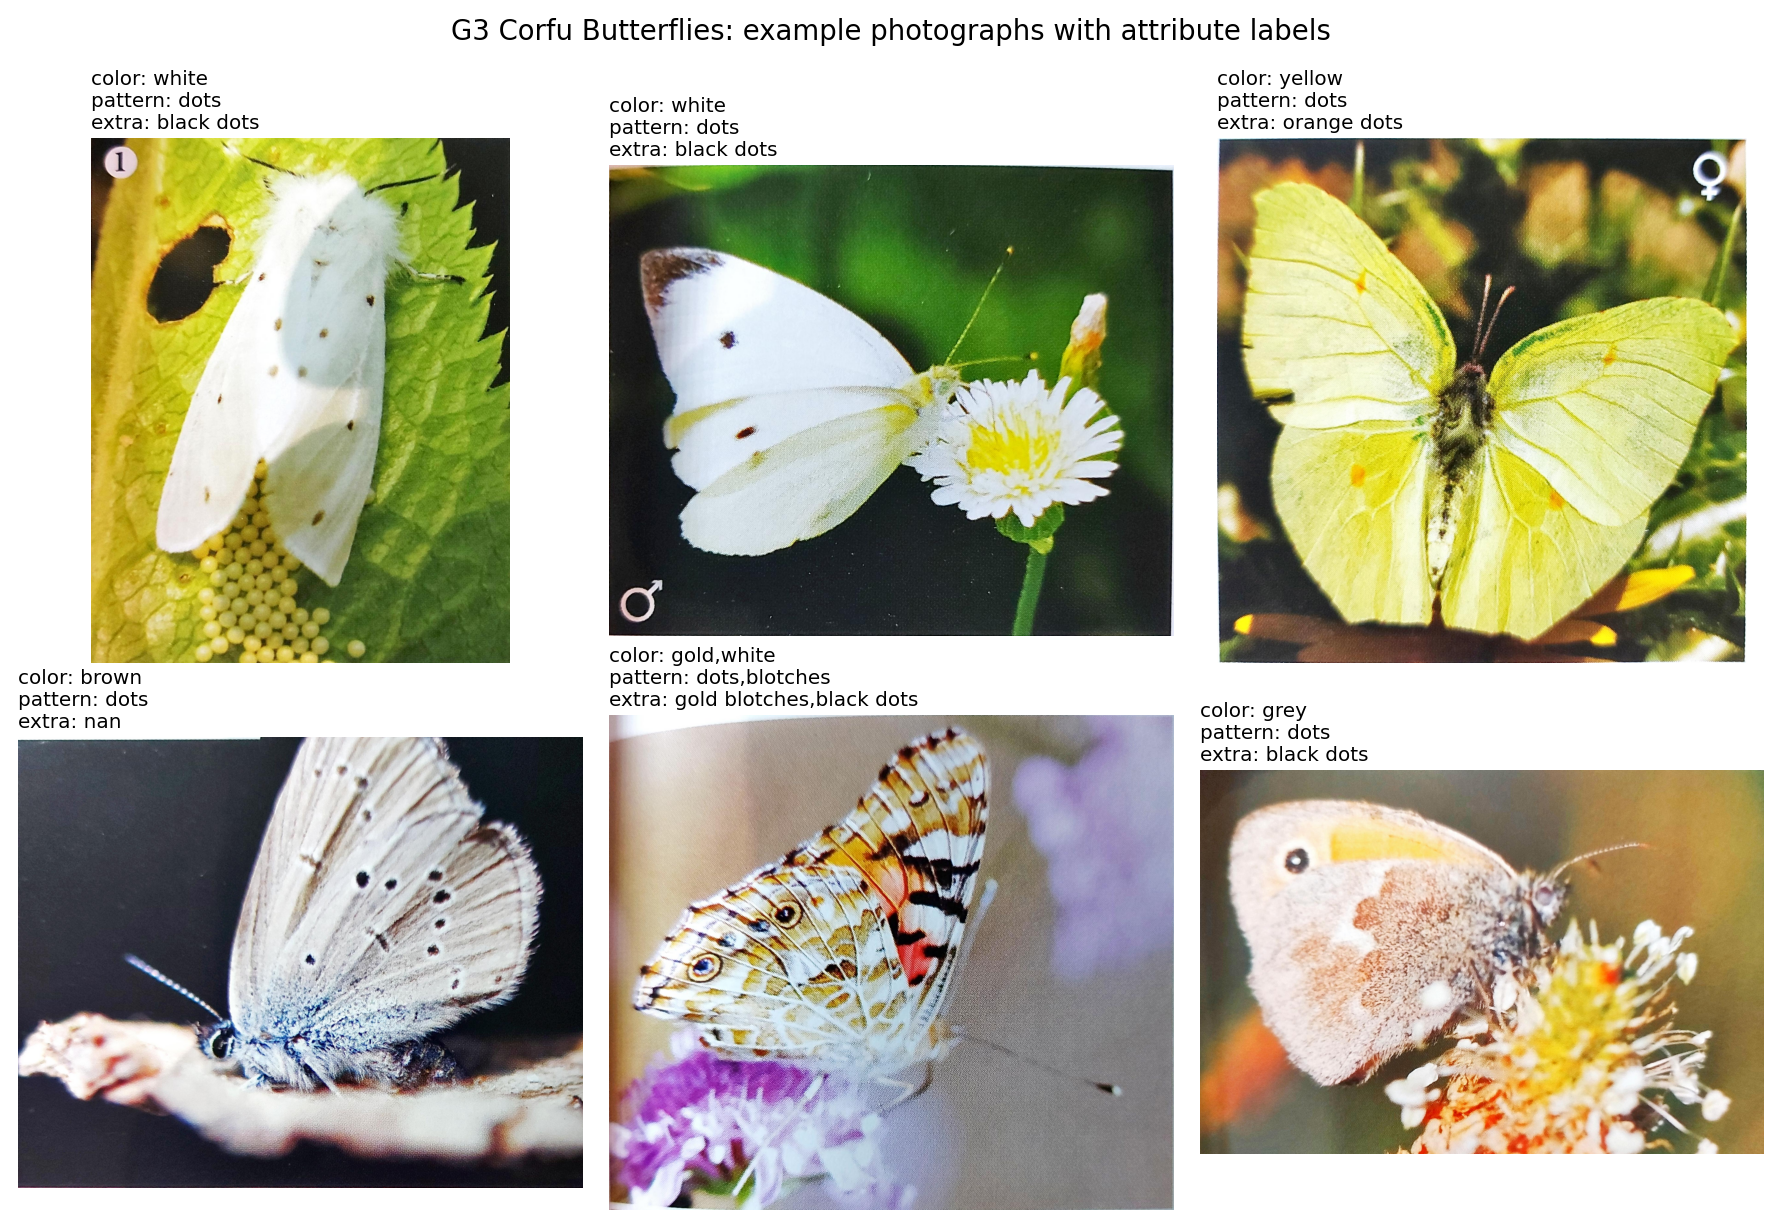
\includegraphics[width=\linewidth]{figures/examples.png}
\caption{Six example photographs from G3 Corfu Butterflies with
their image-level annotation across the three attribute columns
(colour, pattern, extra features). The prediction target is the
45-dimensional multi-hot vector obtained by the union of the three
namespaced token sets.}
\label{fig:examples}
\end{figure}

\subsection{Splits}
Stratified splitting of multi-label data cannot guarantee that every
rare label appears on both sides of a cut. We use the iterative
stratification algorithm~\citep{sechidis2011stratification}
implemented in the \texttt{iterative-stratification} package. A
$15\,\%$ holdout test set (28 images) is drawn first; five
cross-validation folds are then produced over the remaining 137
images. Seed 42 is fixed so that every user obtains bit-identical
splits. Table~\ref{tab:splitsupport} reports the resulting label
support per split.

\begin{table}[t]
\centering
\caption{Label support on the shipped splits. Even under iterative
stratification the 28-image holdout unavoidably covers only a
subset of the 45 labels because many labels appear fewer than five
times in the full corpus. Evaluation-active metrics
(Section~\ref{sec:validation}) therefore average over 24 of 45
labels on the holdout, and we make this explicit in every reported
number.}
\label{tab:splitsupport}
\begin{tabular}{lrr}
\toprule
Split & Images & Labels with $\geq$1 positive \\
\midrule
5-fold training pool & 137 & --- \\
Locked holdout & 28 & 24 of 45 \\
\bottomrule
\end{tabular}

\end{table}

\section{Descriptive Statistics}
\label{sec:stats}

The benchmark is deliberately long-tailed, multi-label, and
small-scale. This section quantifies those three properties so
that users can reason about expected difficulty and choose an
appropriate learning strategy.

\paragraph{Vocabulary composition.}
Table~\ref{tab:namespace} breaks down the 45 labels by attribute
family. The colour namespace dominates the number of positive tokens
per image, followed by \emph{extra features} and then \emph{pattern};
almost every image carries at least one colour and one extra feature
token, while pattern tokens are sparser.

\begin{table}[t]
\centering
\caption{Per-namespace breakdown of the 45-entry label vocabulary.
\textit{Mean positives / image} counts how many labels from that
namespace appear on an average image.}
\label{tab:namespace}
\begin{tabular}{lrrr}
\toprule
Namespace & Labels & Mean positives / image & Total positives \\
\midrule
color & 13 & 1.34 & 221 \\
extra & 26 & 0.96 & 159 \\
pattern & 6 & 1.02 & 169 \\
\bottomrule
\end{tabular}

\end{table}

\paragraph{Label frequency.}
Table~\ref{tab:labeltop} lists the fifteen most frequent labels.
Figure~\ref{fig:longtail} plots the label-frequency rank curve on a
logarithmic scale: the most frequent label covers almost every
image, while a long tail of labels occurs in fewer than five images
each. Rare labels are retained so that macro-averaged metrics reward
performance on the tail, but users that prefer a closed, balanced
subset can subset the vocabulary at any frequency threshold they
choose.

\begin{table}[t]
\centering
\caption{The fifteen most frequent labels in the full 165-image
corpus.}
\label{tab:labeltop}
\begin{tabular}{lrrr}
\toprule
Label & Namespace & Count & Frequency \\
\midrule
dots & pattern & 68 & 0.412 \\
blotches & pattern & 65 & 0.394 \\
brown & color & 62 & 0.376 \\
black dots & extra & 44 & 0.267 \\
white & color & 32 & 0.194 \\
black & color & 29 & 0.176 \\
stripes & pattern & 29 & 0.176 \\
orange & color & 28 & 0.170 \\
yellow & color & 18 & 0.109 \\
black blotches & extra & 18 & 0.109 \\
white blotches & extra & 17 & 0.103 \\
blue & color & 14 & 0.085 \\
grey & color & 14 & 0.085 \\
white stripes & extra & 11 & 0.067 \\
orange blotches & extra & 11 & 0.067 \\
\bottomrule
\end{tabular}

\end{table}

\begin{figure}[t]
\centering
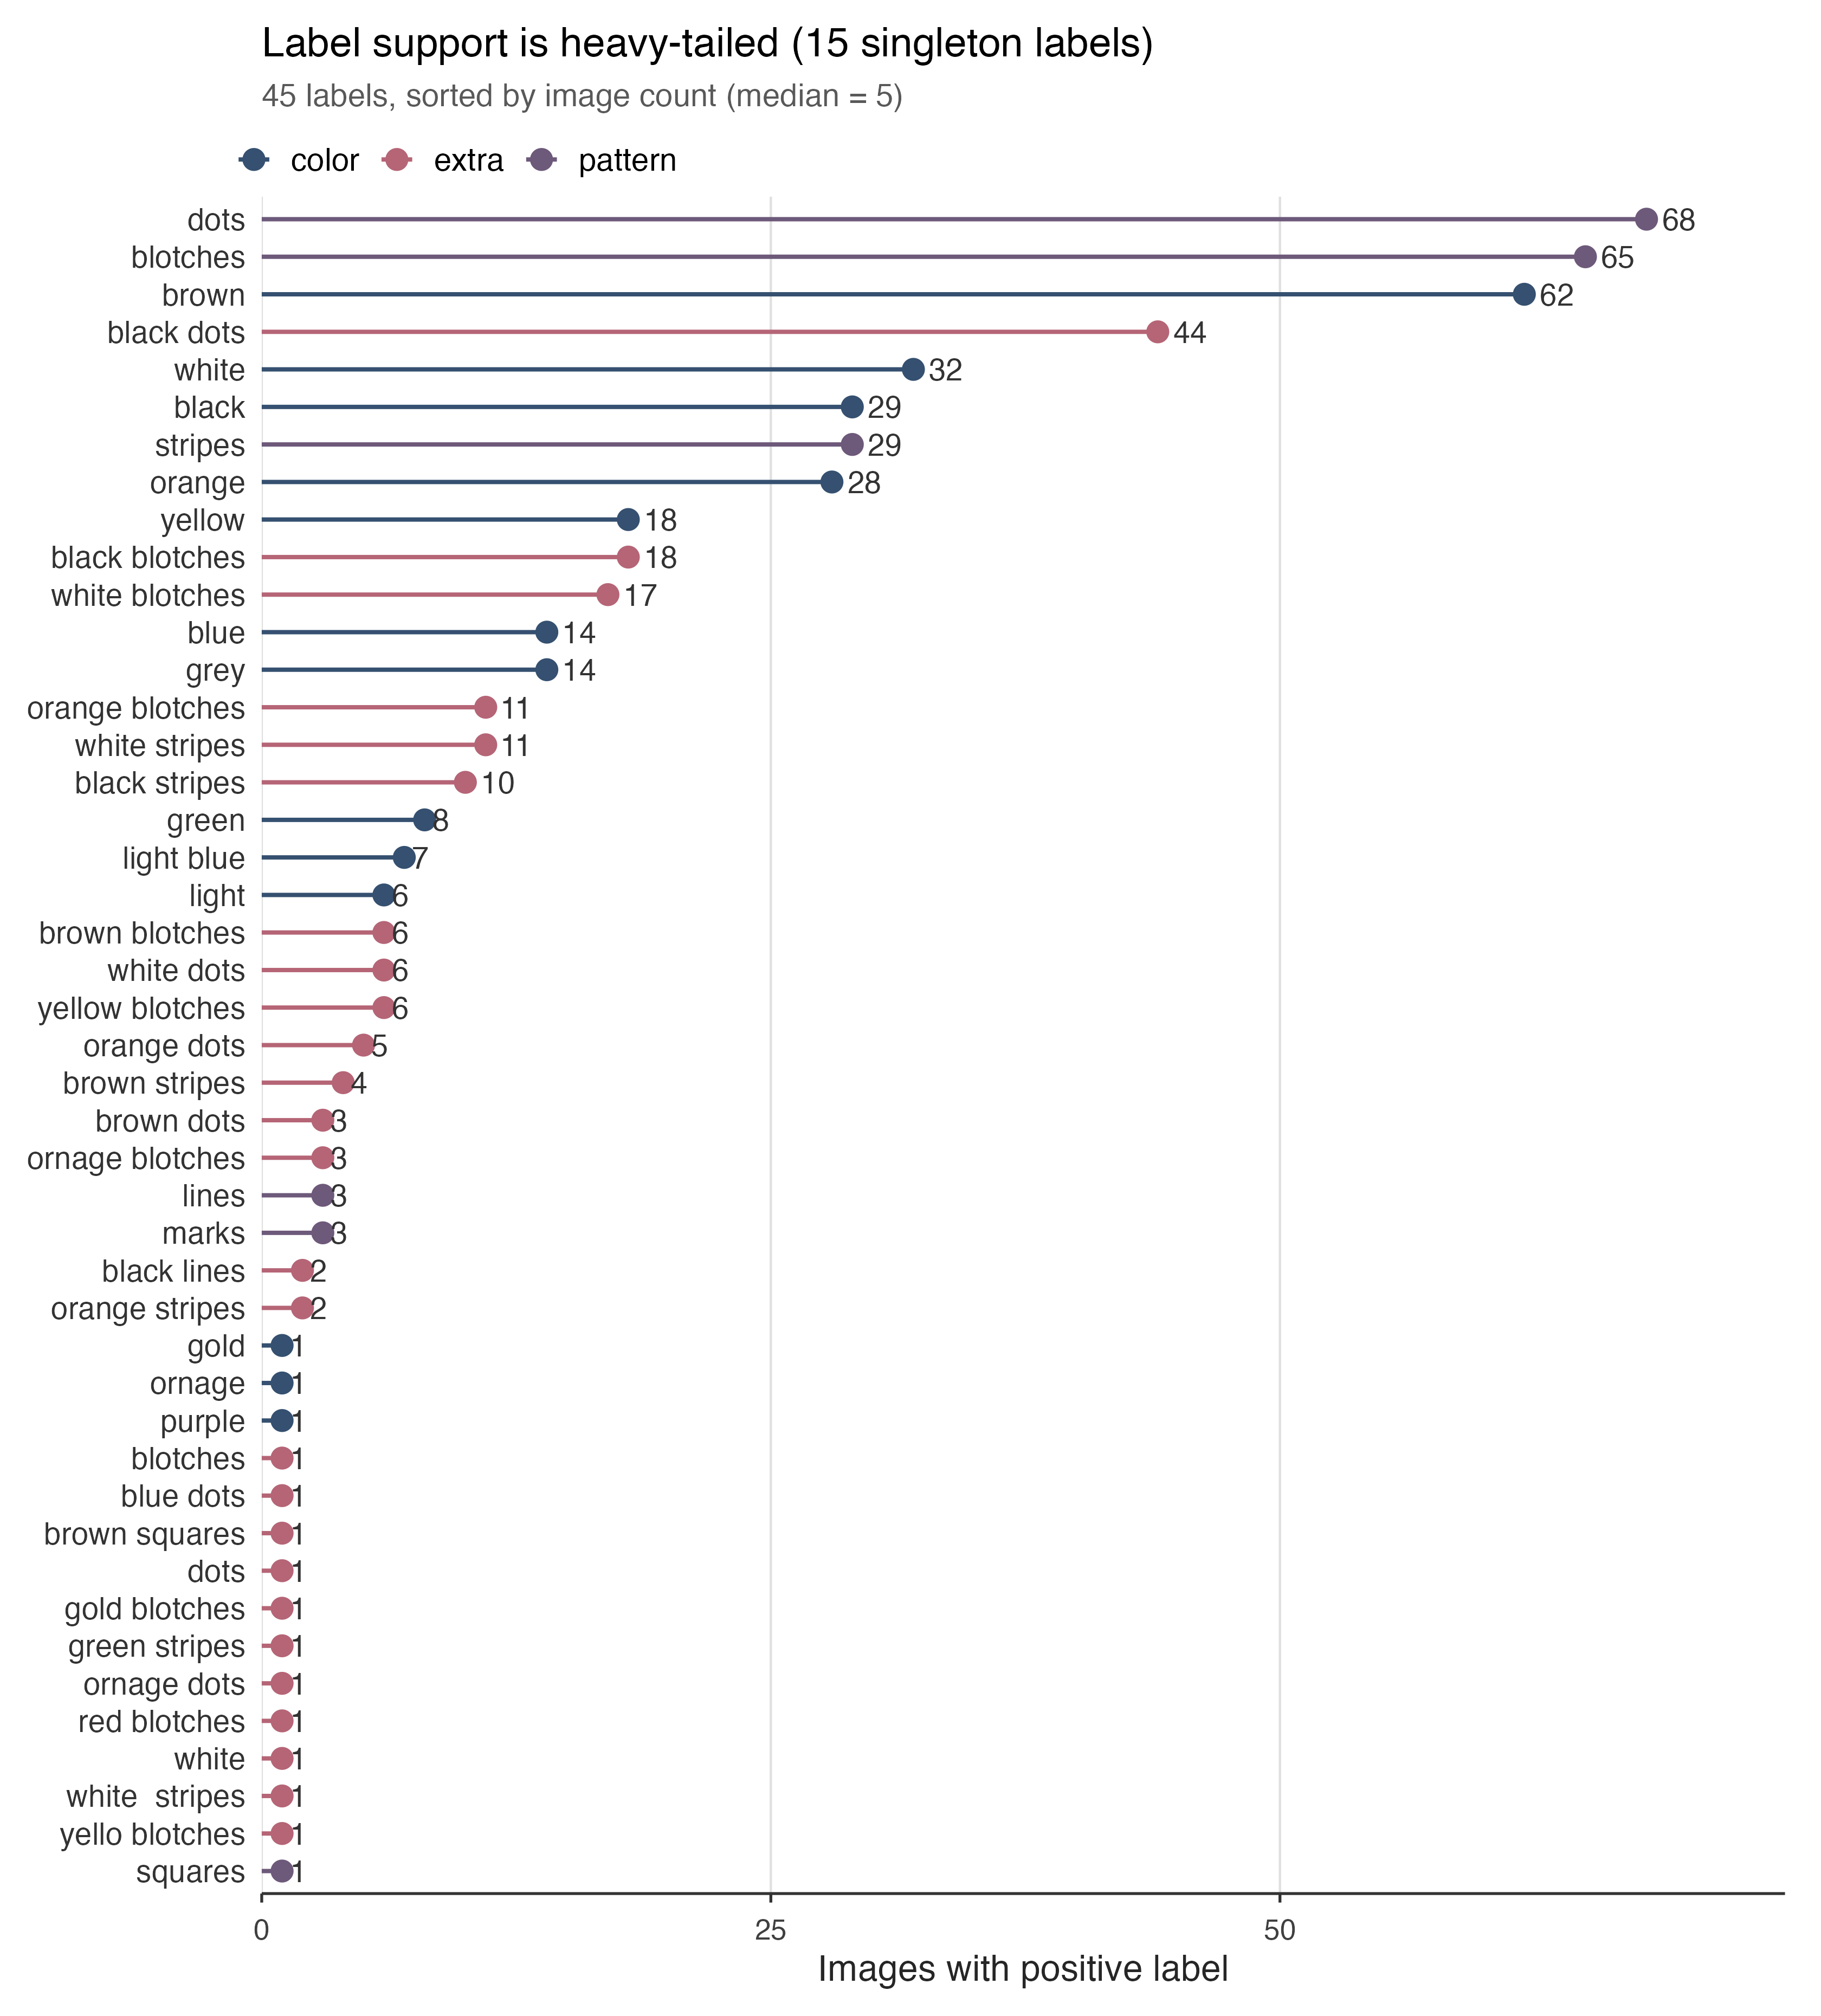
\includegraphics[width=0.85\linewidth]{figures/long_tail.png}
\caption{Label frequency rank curve on a log scale. The steep
decline followed by a long plateau at two to three images per label
is typical of small attribute corpora and a primary reason the
benchmark emphasises macro-F1 alongside micro-F1.}
\label{fig:longtail}
\end{figure}

\paragraph{Label cardinality.}
Figure~\ref{fig:cardinality} shows the distribution of the number
of positive labels per image. Most images carry 2--5 positive
tokens, with very few images at the extremes; the distribution is
approximately Poisson-shaped, consistent with the independent
tokenisation protocol.

\begin{figure}[t]
\centering
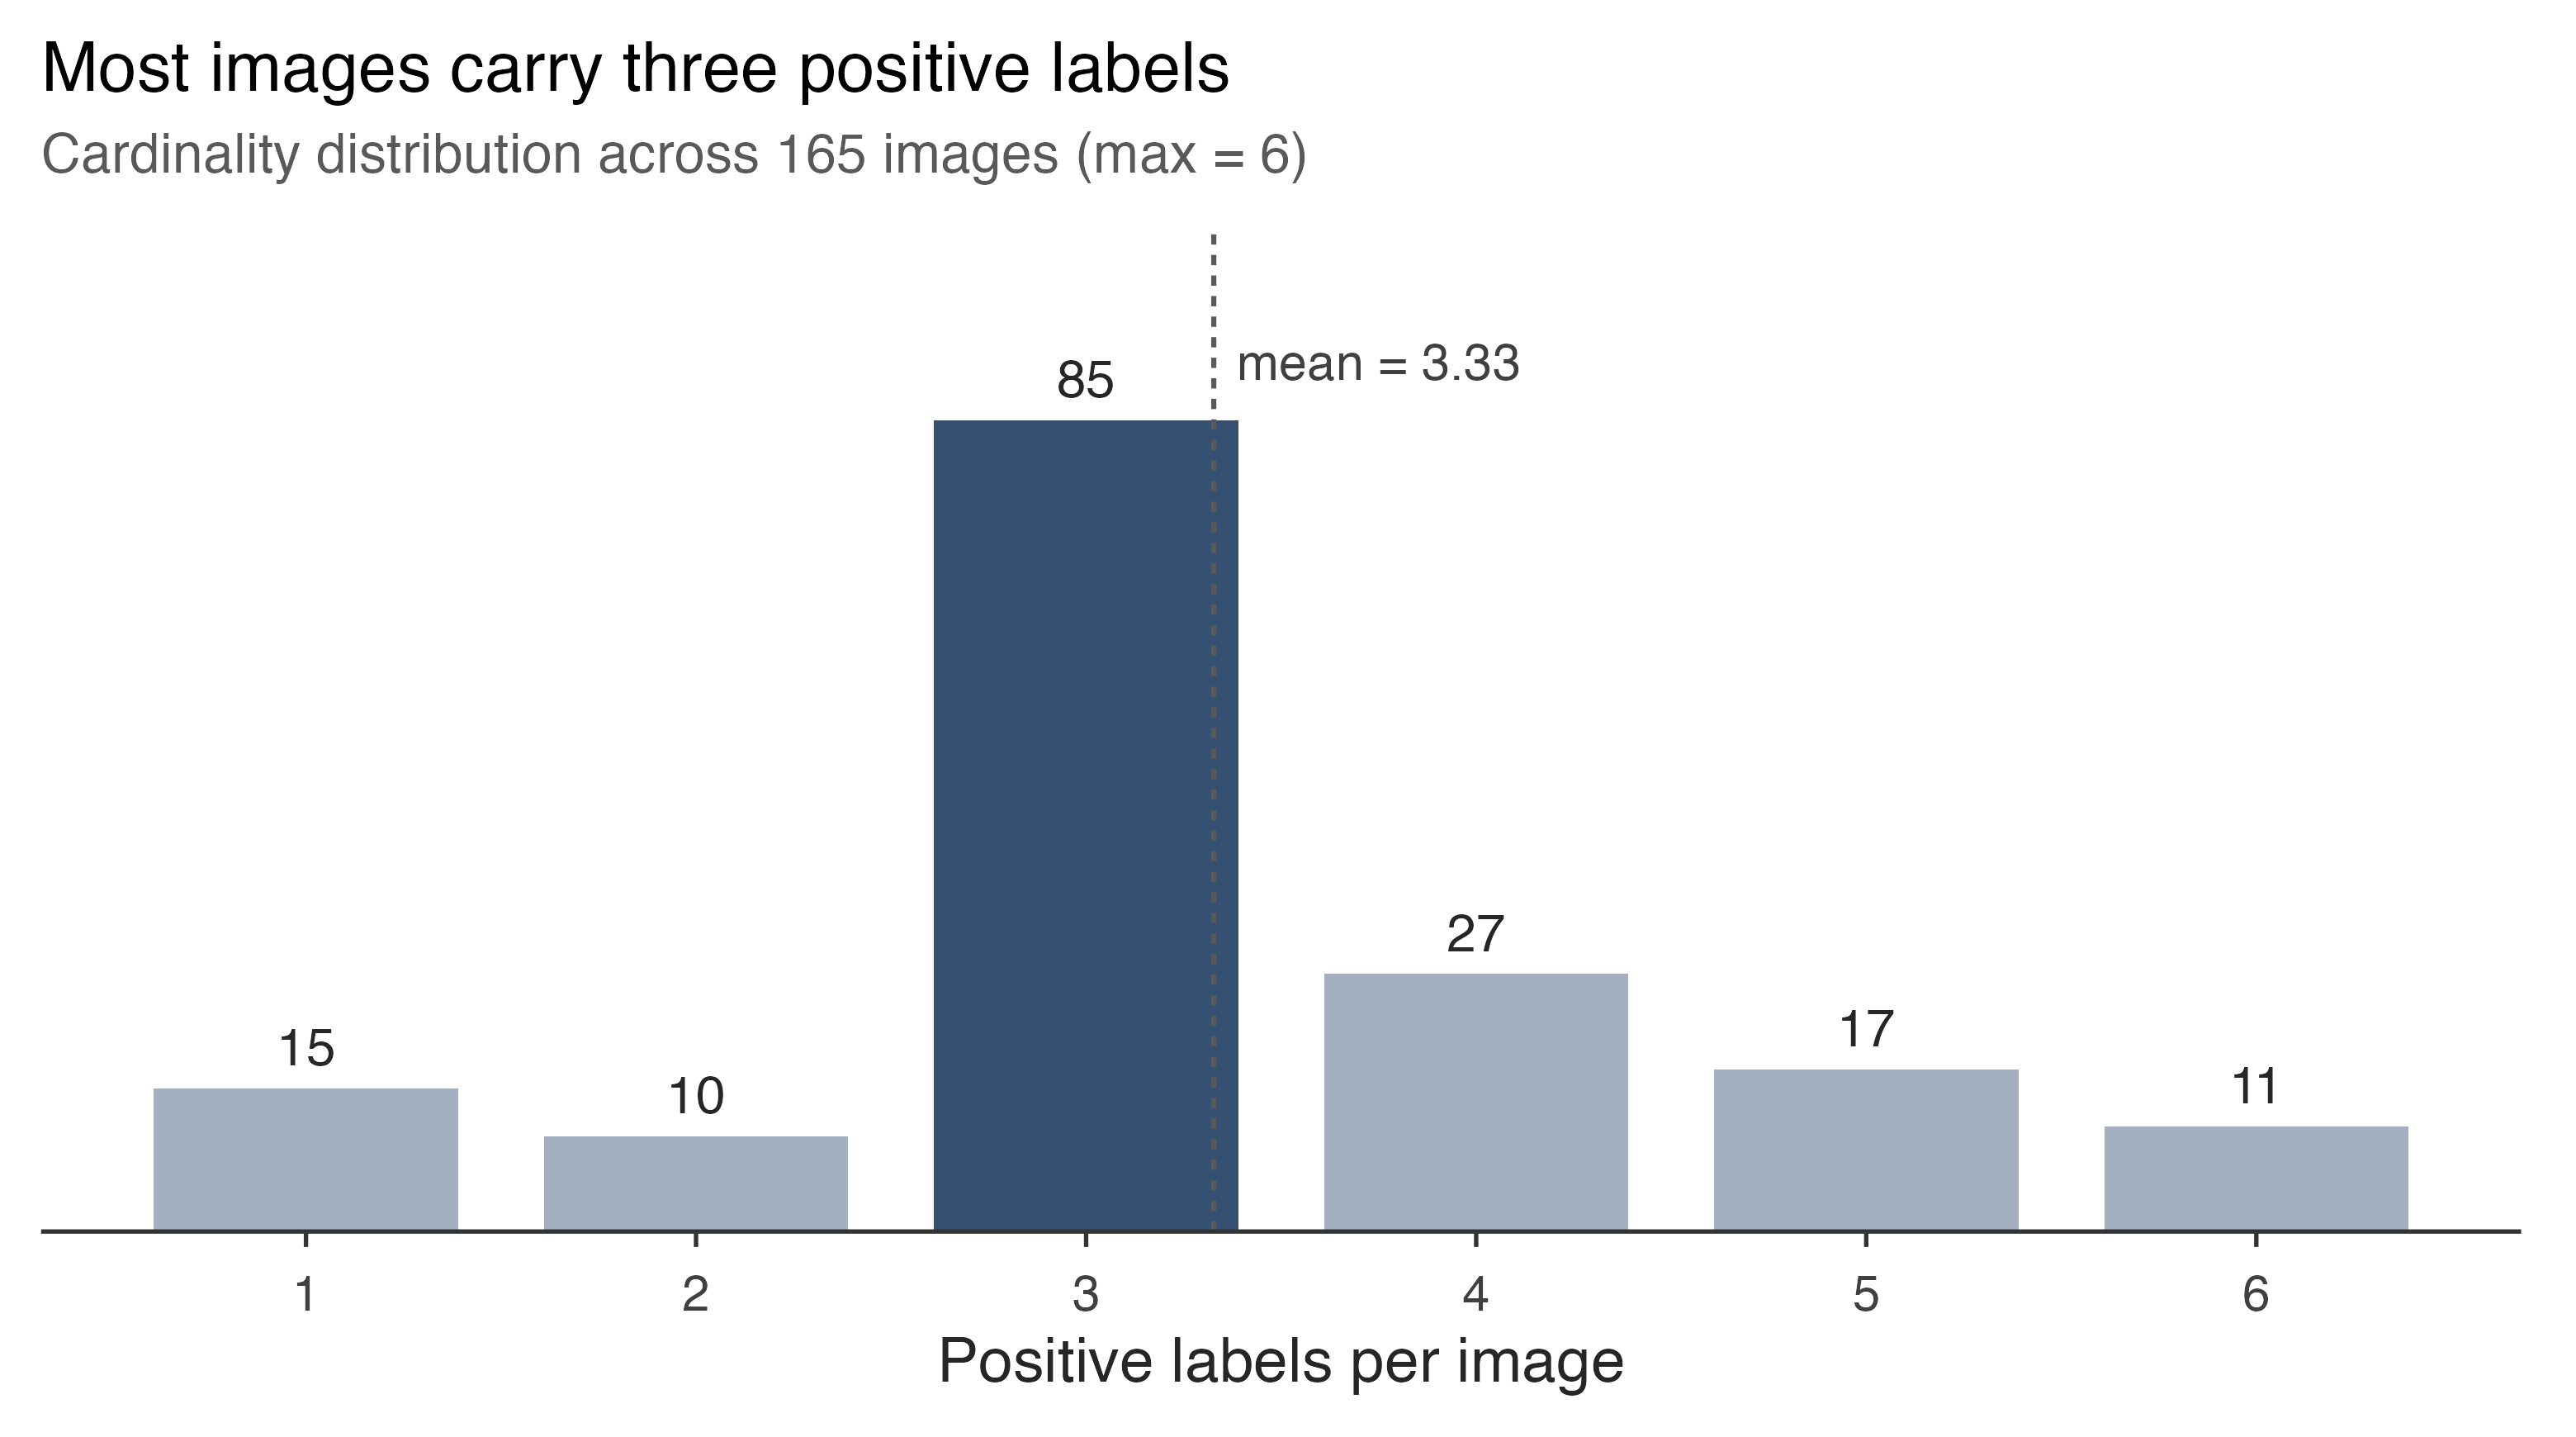
\includegraphics[width=0.8\linewidth]{figures/cardinality.png}
\caption{Distribution of the number of positive labels per image.
The mean cardinality is modest (around three), which makes the
benchmark a tractable multi-label problem: predicting empty
multi-hot vectors or one-label dominant strategies is heavily
penalised by the shipped metrics.}
\label{fig:cardinality}
\end{figure}

\paragraph{Label co-occurrence.}
Figure~\ref{fig:cooccurrence} shows the conditional probability
$P(\text{label}_j \mid \text{label}_i)$ for the fifteen most frequent
labels. Strong off-diagonal entries are expected: colour tokens
co-occur with specific pattern and extra-feature tokens, and
attribute-pair correlations are not uniform. This structure motivates
the benchmark's interest in label-correlation methods as opposed to
pure per-label independent sigmoids.

\begin{figure}[t]
\centering
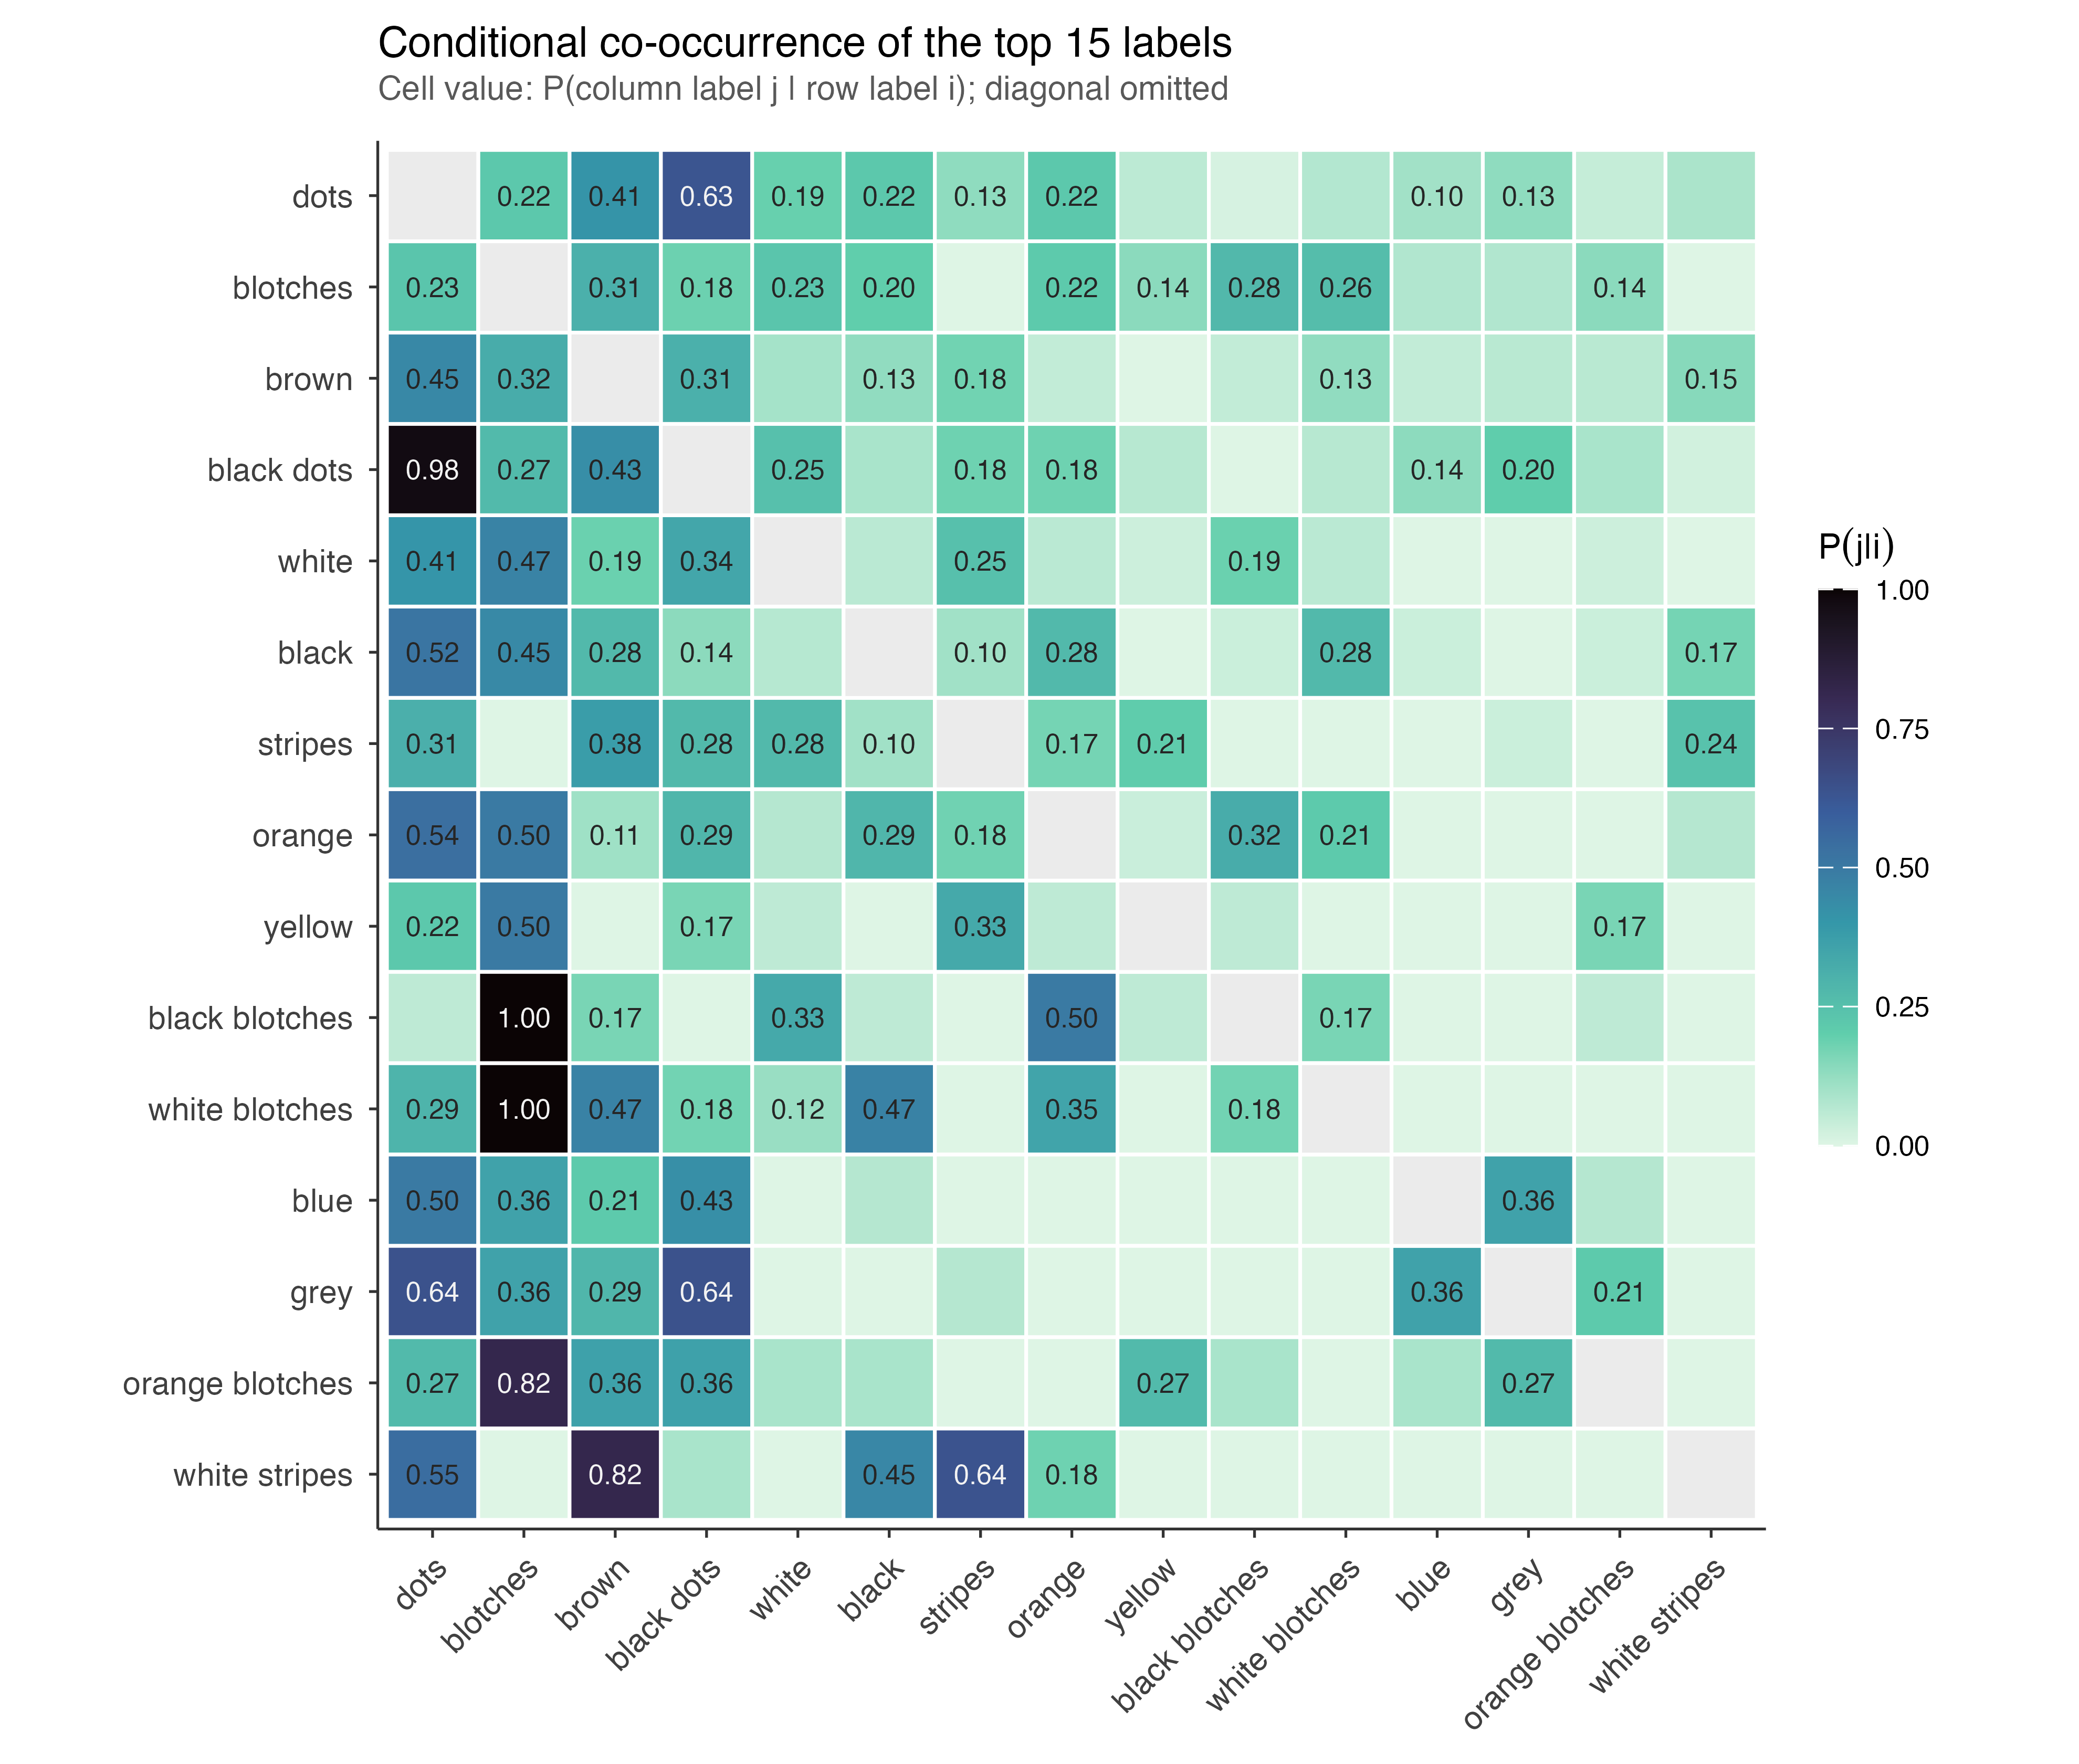
\includegraphics[width=0.85\linewidth]{figures/cooccurrence.png}
\caption{Conditional probability matrix
$P(\text{label}_j \mid \text{label}_i)$ for the fifteen most
frequent labels. The off-diagonal structure is non-trivial and
suggests that methods exploiting label correlations (classifier
chains, GCN-based heads, conditional networks) can plausibly
improve over the independent-sigmoid baseline.}
\label{fig:cooccurrence}
\end{figure}

\section{Reference Baselines and Evaluation Protocol}
\label{sec:validation}

The reference baselines fix the first entry on the benchmark
leaderboard and document the protocol that every subsequent
submission is expected to follow. We release two baselines of
deliberately opposite flavour.

\paragraph{CLIP linear probe.} We encode every image with a frozen
\texttt{open\_clip}~\citep{ilharco2021openclip,cherti2023openclip}
ViT-B/32 visual tower (\texttt{laion2b\_s34b\_b79k} weights from
LAION-2B~\citep{schuhmann2022laion5b}, 512-d normalised features),
and fit class-balanced one-vs-rest logistic-regression heads on each
training fold (\texttt{scikit-learn}~\citep{pedregosa2011scikit},
\texttt{C=1.0}, 2000 iterations, standardised features). Labels with
zero training positives fall back to the empirical mean. The probe
is a cheap, well-known reference~\citep{radford2021clip} that
answers the question of whether a frozen foundation model is already
sufficient.

\paragraph{Fine-tuned ViT-B/16.} We fine-tune a
ViT-B/16~\citep{dosovitskiy2021vit} pre-trained on
ImageNet-1k~\citep{russakovsky2015ilsvrc}. The original classification
head is replaced with a dropout layer ($p=0.1$) and a linear
projection to 45 logits. The loss is binary cross-entropy with
per-class positive weights computed from training-fold frequencies
and clipped to $[0.5, 20]$. Optimisation uses
AdamW~\citep{loshchilov2019adamw}, cosine
schedule~\citep{loshchilov2017sgdr}, learning rates
$3\times10^{-5}$ (backbone) and $10^{-3}$ (head), weight decay
$0.05$, batch size 16, and 30 epochs. Augmentations include random
resized crop to $224\times224$, horizontal flip, colour jitter, and
RandAugment~\citep{cubuk2020randaugment} (2 ops, magnitude 7);
inputs are normalised with ImageNet statistics and gradients are
clipped to an $\ell_2$ norm of 1.0.

\paragraph{Protocol.} For each of the 5 folds the model is trained
on the four training splits and validated on the held-out fifth.
The checkpoint with the highest validation macro-F1 is retained.
The five fold-best checkpoints are then scored on the locked
holdout individually and as a logit-averaged ensemble.

\paragraph{Metrics.} Macro-F1 on the locked holdout ensemble is the
primary benchmark metric. We also report micro-F1, exact-match
accuracy, mean AUROC, and mean average precision. Macro-F1 is
averaged over the \emph{evaluation-active} labels (those with at
least one positive in the evaluation set: 24 of 45 on the holdout,
about 32 of 45 on a typical validation fold); the remaining labels
contribute only to micro metrics. Zero-support labels are
documented in Table~\ref{tab:splitsupport}.

\paragraph{Reference results.}
Table~\ref{tab:baseline} reports both baselines side by side.

\begin{table}[t]
\centering
\caption{Reference baselines on G3 Corfu Butterflies. The frozen
CLIP linear probe establishes the out-of-the-box foundation-model
number; the fine-tuned ViT-B/16 improves macro-F1 by $+10.4$
($+8.6$) points on cross-validation (holdout ensemble),
demonstrating that the benchmark rewards representation learning
beyond a frozen probe.}
\label{tab:baseline}
\begin{tabular}{lcccc}
\toprule
 & \multicolumn{2}{c}{5-fold CV} & \multicolumn{2}{c}{Locked holdout} \\
\cmidrule(lr){2-3}\cmidrule(lr){4-5}
Metric & CLIP probe & ViT-B/16 FT & CLIP probe & ViT-B/16 FT \\
\midrule
Macro-F1 & 0.291 $\pm$ 0.046 & 0.395 $\pm$ 0.040 & 0.256 & 0.342 \\
Micro-F1 & 0.510 $\pm$ 0.032 & 0.525 $\pm$ 0.016 & 0.400 & 0.563 \\
Exact match & 0.050 $\pm$ 0.048 & 0.029 $\pm$ 0.027 & 0.071 & 0.000 \\
Mean AUROC & 0.233 $\pm$ 0.026 & 0.209 $\pm$ 0.026 & 0.358 & 0.225 \\
Mean AP & 0.490 $\pm$ 0.040 & 0.528 $\pm$ 0.015 & 0.406 & 0.443 \\
\bottomrule
\end{tabular}

\end{table}

Three observations follow from Table~\ref{tab:baseline}. First, the
fine-tuned ViT-B/16 outperforms the frozen CLIP probe on macro-F1
and micro-F1, as expected but not guaranteed at this scale. Second,
the absolute macro-F1 is below $0.5$: the benchmark is neither
saturated nor trivially solved, leaving meaningful headroom for
methodological contributions. Third, exact-match accuracy is near
zero for both baselines, which is consistent with the cardinality
distribution in Figure~\ref{fig:cardinality}: correctly predicting
the exact multi-hot vector is hard when the expected number of
positives is around three.

\paragraph{Rules for comparability.} A valid submission must
(i)~use the shipped \texttt{splits/} without modification,
(ii)~train only on the training folds when reporting
cross-validation, (iii)~touch the holdout exactly once, at final
evaluation, and (iv)~report all five metrics in
Table~\ref{tab:baseline}. The reference implementations satisfy
these rules and serve as templates.

\section{Usage Notes}

\paragraph{Reproduction.} The benchmark is reproduced by four
commands documented in \texttt{BENCHMARK.md}:
\texttt{prepare\_dataset.py}, \texttt{g3.train},
\texttt{g3.holdout\_eval}, and \texttt{export\_results.py}. The CLIP
linear probe is an additional one-liner
(\texttt{g3.clip\_baseline}). The recommended fast path is a free
Colab or Kaggle GPU notebook: a full 5-fold fine-tuning run with
mixed precision finishes in roughly fifteen minutes. A ready-to-run
notebook, \texttt{notebooks/colab\_quickstart.ipynb}, is shipped
with the release. The same pipeline runs unchanged on commodity
CPUs in about one hour.

\paragraph{Extension.} The vocabulary
(\texttt{data/label\_vocab.json}) and the classification head
(\texttt{src/g3/model.py}) are decoupled. Additional label fields
(species, lifecycle, habitat) can be added by appending columns to
\texttt{metadata.csv} and extending the vocabulary; the pipeline is
label-agnostic. Subsets can be obtained by frequency thresholding
the vocabulary file directly.

\paragraph{Limitations.}
\begin{enumerate}
  \item \textbf{Scale.} 165 images is small by modern deep-learning
        standards; the benchmark is positioned as a small-data
        regime rather than a pre-training corpus.
  \item \textbf{Holdout coverage.} The 28-image locked holdout
        evaluates 24 of 45 labels. We report metrics on the
        evaluation-active subset to avoid inflating averages with
        zero-support labels.
  \item \textbf{Annotator count.} A small team produced the
        annotations; inter-annotator agreement is not yet reported.
  \item \textbf{Image-level only.} No region-level masks, bounding
        boxes, or keypoints are included. Species labels are not
        provided.
\end{enumerate}

\section{Future Work}
Three extensions are of particular interest from a computer-vision
perspective. \emph{First}, a held-out second-annotator pass would
quantify label reliability (Cohen's $\kappa$ per namespace) and
place upper bounds on achievable macro-F1. \emph{Second}, weak
region-level annotations (wing/body/antennae bounding boxes) would
enable localised attention studies and weakly-supervised
segmentation on the same images. \emph{Third}, the reference
implementation currently targets CPU and CUDA reliably; the Apple
Silicon MPS backend in PyTorch~2.11~\citep{paszke2019pytorch}
exhibits numerical
instabilities on some fold seeds, and a validated
\texttt{--device mps} path is on our roadmap.

\section{Code Availability}
\begin{itemize}
  \item \textbf{Dataset:} Harvard Dataverse,
        \href{https://doi.org/10.7910/DVN/W6UMIR}{DOI 10.7910/DVN/W6UMIR}
        (CC~BY~4.0).
  \item \textbf{Code:} MIT-licensed, distributed alongside the
        data under \texttt{src/g3/} and \texttt{scripts/}.
        Installation and reproduction instructions are in
        \texttt{README.md} and \texttt{BENCHMARK.md}.
\end{itemize}

\section*{Dedication and Acknowledgements}
This dataset is dedicated to the memory of Professor Markos Avlonitis, whose sustained contributions to the
computational study of biodiversity in the Ionian Islands shaped
both the scientific culture in which this work was carried out and
the motivation to build open, reusable resources of this kind. The
authors also thank the Corfu Butterfly Conservation community for
supporting the field work that produced the images.

\clearpage
\bibliographystyle{plainnat}
\bibliography{references}

\end{document}
